
\section{La Celda LSTM}


\begin{frame}
	\frametitle{La Celda LSTM}
	\vspace{-2mm}
	\begin{center}
		\begin{tikzpicture}[
			% Estilos de los nodos
			cellnode/.style={draw=none, rectangle, minimum height=3cm, minimum width=4cm, fill=pink!50},
			statenode/.style={draw=none, minimum height=1cm, minimum width=2cm, fill=yellow!30, xshift=-1cm},
			labelnode/.style={draw=none},
			% Estilo de las flechas
			arrowstyle/.style={->, thick, >=stealth}
			]
			
			% Nodo de estado
			\node[cellnode] (lstm) {LSTM};
			\node[statenode] (state) [above=0 of lstm] {};
			\node[labelnode] (statelabel) [above right=-0.5 and 1 of state, xshift=80] {};
			\node at (-0.38, 2.5) {Celda de Estado (Cell State)};
			
			
			% Nodos de entrada y salida
			\node[labelnode] (ht) at (0,4) {$\hat{y}_t$};
			\node[labelnode] (at1) [left=2cm of lstm] {$\vec{h}_{t-1}$};
			\node[labelnode] (ct1) at (-3,1.7) {$c_{t-1}$};
			\node[labelnode] (xt) [below=of lstm] {$\vec{x}_t$};
			\node[labelnode] (at) [right=2cm of lstm] {$\vec{h}_t$};
			\node[labelnode] (ct) at (3,1.7) {$c_t$};
			
			% Flechas
			\draw[arrowstyle] (xt) -- (lstm);
			\draw[arrowstyle] (lstm) -- (ht);
			\draw[arrowstyle] (at1) -- (lstm);
			\draw[arrowstyle] (ct1) -| (lstm.north west);
			\draw[arrowstyle] (lstm.north east) -- ++(right:0cm) |- (ct);
			\draw[arrowstyle] (lstm) -- (at);
			
			% Rectángulo punteado alrededor del estado
			\begin{scope}[on background layer]
				\node[draw=black!60, dashed, thick, fill=yellow!20, fit=(state) (statelabel), inner sep=0.3cm, xshift=-1cm] (statebox) {};
			\end{scope}
			
		\end{tikzpicture}
	\end{center}
	
\end{frame}


\begin{frame}
	\frametitle{Elementos de la Celda LSTM}
	\begin{itemize}
		\item Los elementos $\vec{h}_{t-1}, \vec{h}_{t}, \vec{\hat{y}}_{t}, \vec{x}_{t}$ tienen la misma función que en una RNN.
		\item La Red LSTM incorpora una nueva funcionalidad a diferencia de una RNN convencional: la celda de estado (Memoria a largo plazo).
		\item La entrada $c_{t-1}$ almacena información de la memoria a largo plazo, que puede ser de utilidad para la Red Neuronal.
		\item La salida $c_{t}$ contiene información actualizada para la memoria a largo plazo.
	\end{itemize}
\end{frame}

\begin{frame}
	\frametitle{Elementos de la Celda LSTM}
	Una Red LSTM cuenta con \textit{cuatro redes neuronales} diferentes en su interior, que en la literatura se asocian cuatro compuertas:
	
	\begin{itemize}
		\item \textbf{\textit{Forget Gate:}} Decide qué información de la memoria a largo plazo se recuerda o se olvida ($c_{t-1}$).
		\item \textbf{\textit{Candidate memory:}} Presenta elementos candidatos de la memoria a corto plazo para formar parte de la memoria a largo plazo ($c_{t}$).
		\item \textbf{\textit{Update Gate:}} Actualiza la memoria a largo plazo, seleccionando los mejores candidatos de los presentados por la \textbf{\textit{Candidate memory.}}
		\item \textbf{\textit{Output Gate:}} Decide qué información del estado anterior ($h_{t-1}$) y de las entradas actuales vale la pena llevar a la memoria a corto plazo ($h_{t}$).
	\end{itemize}
\end{frame}



\begin{frame}
	\frametitle{Ejemplito: Predictor de consumo de energía eléctrica}
	\vspace{-5mm}
	
	\begin{center}
		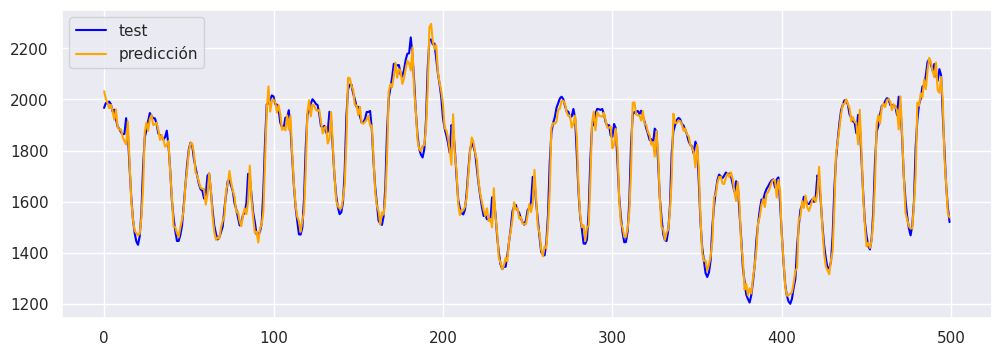
\includegraphics[width=0.7\linewidth]{pred1.png}
		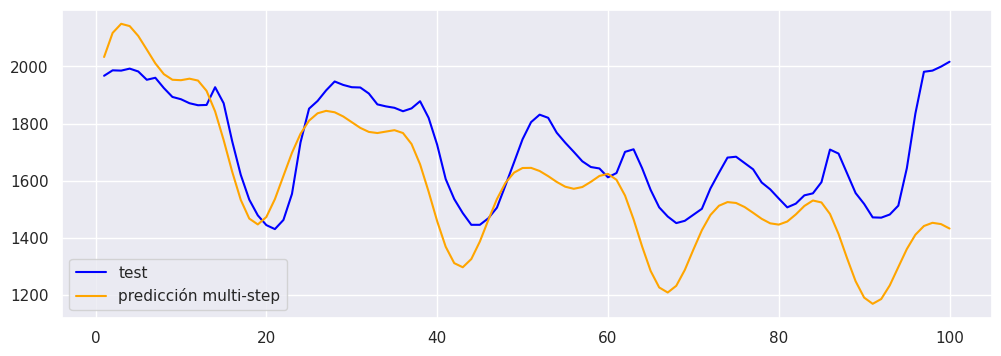
\includegraphics[width=0.7\linewidth]{pred2.png}
	\end{center}
\end{frame}
